\section{Zielsetzung}
\label{sec:Zielsetzung}
Das Ziel des Versuches ist das Bestimmen verschiedener ohmscher Widerstände, Kapazitäten und Induktivitäten durch ausgewählte Brückenschaltungen. Außerdem werden 
durch den Versuch das Verständnis der Kirchhoffschen Gesetze vertieft und verschiedene Brückenschaltungen vorgestellt.  

\section{Theorie}
\label{sec:Theorie}
    \subsection{Funktionsprinzip einer Brückenschaltung}
    Die Funktionsweise einer Brückenschaltung beruht auf zwei Kirchhoffschen Gesetzen. Die sogenannte Knotenregel besagt, dass an einem Knotenpunkt die Summe der 
    zufließenden Ströme der Summe der abfließenden Ströme entsprechen muss. Zufließende Ströme haben ein positives Vorzeichen und abfließende Ströme haben ein 
    negatives Vorzeichen. Dann gilt 
    \begin{equation}
        \label{eqn:Knotenregel}
        \sum_k {I_k} = 0 \,.
    \end{equation}
    $I_k$ sind dabei die einzelnen zufließende oder abfließende Ströme. 
    Die sogenannte Maschenregel beschreibt, dass die Summe aller treibenden, elektrischen Spannungen der Summe der abfallenden Spannungen innerhalb einer beliebigen, geschlossenen 
    Masche eines Stromkreises entspricht. Dabei haben die abfallenden Spannung ein negatives Vorzeichen und die treibenden Spannungen ein positives Vorzeichen. 
    Dann gilt
    \begin{equation}
        \label{eqn:Maschenregel}
        \sum_k {U_k} = 0 
    \end{equation}
    innerhalb einer Masche. $U_k$ sind dabei die in der Masche treibenden oder abfallenden Spannungen. 
    Diese beiden Regel können verwendet werden, um Schaltpläne zu erstellen, die es ermöglichen die Kenngrößen unbekannter Bauteile zu bestimmen. Eine 
    solche prinzipielle Brückenschaltung ist in Abbildung (\ref{pic:prinzipielle_Brückenschaltung}) zu sehen. $R$ bezeichnet ohmsche Widerstände.
    \begin{figure}[H]
        \centering
        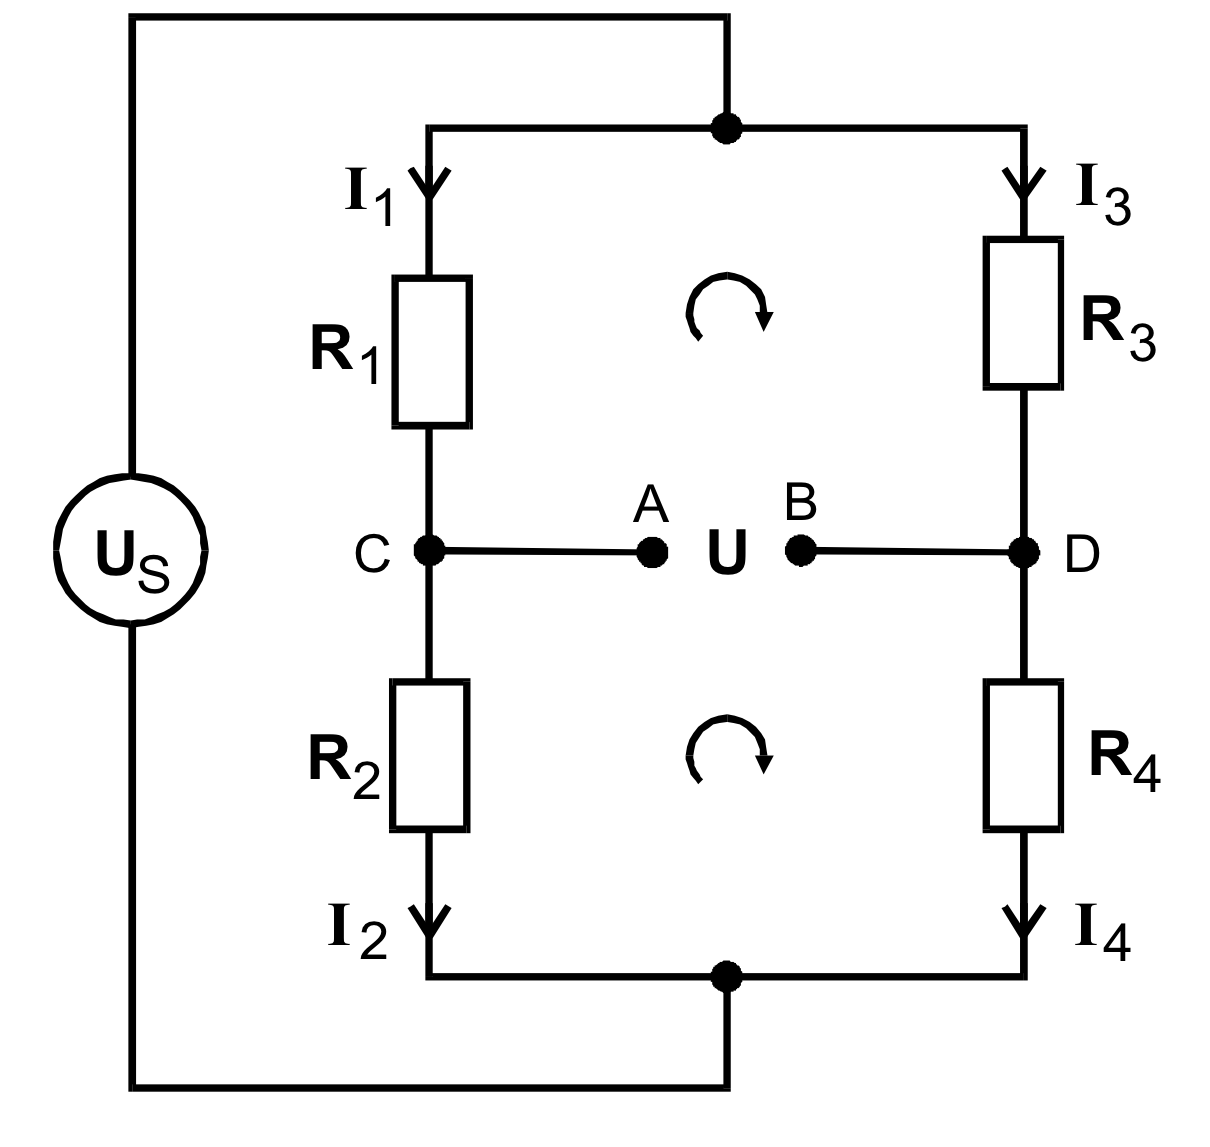
\includegraphics[width=0.4\linewidth]{prinzipielle_Schaltung.png}
        \caption{Schaltplan einer prinzipiellen Brückenschaltung}
        \label{pic:prinzipielle_Brückenschaltung}
    \end{figure}
    Die unbekannte Kenngröße wird durch die sogenannte Nullmethode bestimmt. Bei dieser wird $R_2$ variiert bis zwischen Punkt A und Punkt B keine Spannung mehr zu
    messen ist. 
    \subsection{Wheatstonesche Brücke}
    In der Whaeatstoneschen Brückenschaltung werden jeweils zwei in Reihe geschaltete ohmsche WIderstände parallel zueinander geschaltet, wie im Schaltplan in Abbildung 
    (\ref{pic:Wheatstonesche_Brueckenschaltung}) zu sehen. 
    Die Wheatstonesche Brückenschaltung wird verwendet, um einen unbekannten ohmschen Widerstand $R_x$ zu bestimmen. Dies erfolgt durch die Formel 
    \begin{equation}
        \label{eqn:Wheatstone_R}
        R_x = R_2 \cdot \frac{R_3}{R_4} \,.
    \end{equation}
    \subsection{Kapazitätsmessbrücke}
    Die Kapazitätsmessbrücke wird zur Bestimmung der Kenngrößen eines Kondensators mit Kapazität $C_x$ und ohmschen Widerstand $R_x$ genutzt. In dieser Schaltung 
    wird der Widerstand $R_2$ der Wheatstoneschen Brücke durch einen Kondensator mit Kapazität $C_2$ und ohmschen Widerstand $R_2$ ersetzt. Die unbekannte Kapazität
    wird durch 
    \begin{equation}
        \label{eqn:Kapazitaet_C}
        C_x = C_2 \cdot \frac{R_4}{R_3} \,.
    \end{equation}
    berechnet. Der unbekannte ohmsche Widerstand wird mithilfe der Formel (\ref{eqn:Wheatstone_R})
    %\begin{equation}
    %    \label{eqn:Kapazitaet_R}
    %    R_x = R_2 \cdot \frac{R_3}{R_4} \,.
    %\end{equation}
    berechnet. 

    \subsection{Induktivitätsmessbrücke}
    Mithilfe der Induktivitätsmessbrücke werden die Kenngrößen einer unbekannten Spule mit Induktivität $L_x$ und $R_x$ berechnet. Im Vergleich zum Schaltbild der Kapazitätsmessbrücke
    wird der Kondensator mit Kapazität $C_2$ und ohmschen Widerstand $R_2$ durch eine Spule mit Induktivität $L_2$ und $R_2$ ersetzt. Die Induktivität $L_x$ wird 
    mithilfe der Formel 
    \begin{equation}
        \label{eqn:Induktivität_L}
        L_x = L_2 \cdot \frac{R_3}{R_4} \,.
    \end{equation}
    berechnet. Der ohmsche Widerstand $R_x$ wird wie die vorherigen mithilfe der Formel (\ref{eqn:Wheatstone_R}) berechnet. 
    \subsection{Maxwell-Brücke}
    Die Maxwell-Brücke wird wie die Induktivitätsmessbrücke zur Messung von Induktivität verwendet. Der Schaltplan ist in Abbildung (\ref{pic:Maxwell-Bruecke}) zu sehen. 
     Die unbekannte Induktivität $L_x$ wird durch 
    \begin{equation}
        \label{eqn:Induktivität_L_Maxwell}
        L_x = R_2 \cdot R_3 \cdot C_4 
    \end{equation}
    berechnet. Für $R_x$ gilt Formel (\ref{eqn:Wheatstone_R}). 
    \subsection{Wien-Robinson-Brücke}
    Das Schaltbild der Wien-Robinson-Brücke ist in Abbildung (\ref{pic:WRB}) zu sehen. In dieser Schaltung gibt es kein Abgleichelement, stattdessen fungiert die 
    Schaltung als elektrischer Filter. Die Schwingung mit der Frequenz 
    \begin{equation}
        \omega_0 = \frac{1}{R \cdot C}
        \label{eqn:omega_0}
    \end{equation}
   wird geschwächt. Mit der Brückenspannung $U_{\text{Br}}$ und der Quellspannung $U_{\text{S}}$ gilt
    \begin{align}
    \left| \frac{U_{\text{Br}}}{U_{\text{S}}}\right| &= \sqrt{\frac{1}{9} \cdot \frac{(\Omega² - 1)²}{(1-\Omega²)² + 9\Omega²}} & \text{mit} \,\, \Omega &= \frac{\omega}{\omega_0} \, .
    \label{eqn:Omega}
    \end{align}

    \subsection{Kirrfaktor}
    Der Klirrfaktor $k$ ist ein Qualitätsmaß für Sinusschwingungsgeneratoren, da dieser darstellt, wie fehlerbehafteten die vom Generator erzeugte Sinusspannung ist. 
    Dieser Faktor wird mithilfe des Verhältnisses der Sinusschwingung mit der Überlagerungsschwingung bestimmt und berechnet sich durch 
    \begin{align}
        k = \frac{1}{U_1} \sqrt{\sum_i ^n {{U_i}²}} \, .
    \label{eqn:Klirrfaktor}
    \end{align}
    
    %\subsection{Fehlerrechnung}
    %Im Folgenden werden Mittelwerte von Messungen gebildet. Diese Mittelwerte werden durch 
    %$$\bar{x} = \frac{1}{n} \cdot \sum_{i = 1}^{n}x_i$$ berechnet. $n$ ist dabei die Anzahl der Messungen aus welcher der Mittelwert bestimmt wird und
    %$x_{i}$ beschreibt die einzelnen Messdaten.
    %Der Mittelwertsfehler wird durch 
    %$$\Delta \bar{x} = \sqrt{\frac{1}{n \cdot (n - 1)} \cdot \sum_{i = 1}^{n}(x_i - \bar{x})} $$
    %berechnet. Bei Größen, die von mehreren fehlerbehafteten Größen abhängig sind, wird die Gaußsche Fehlerfortpflanzung 
    %$$\Delta f = \sqrt{\sum_{i = 1}^{n} \left( \frac{\partial f}{\partial x_i} \right)^2 \cdot \left(\Delta x_i \right)^2}$$
    %zur Berechnung des Fehlers verwendet. \\


